\documentclass[a4paper]{article}

%% Language and font encodings
\usepackage[english]{babel}
\usepackage[utf8x]{inputenc}
\usepackage[T1]{fontenc}

%% Sets page size and margins
\usepackage[a4paper,top=3cm,bottom=2cm,left=3cm,right=3cm,marginparwidth=1.75cm]{geometry}

%% Useful packages
\usepackage{listings}
\usepackage{amsmath}
\usepackage{pdfpages}
\usepackage{graphicx}
\usepackage[colorinlistoftodos]{todonotes}
\usepackage[colorlinks=true, allcolors=blue]{hyperref}

\definecolor{lightgrey}{rgb}{0.9, 0.9, 0.9}
\lstset{ %
    backgroundcolor=\color{lightgrey}}

\title{Distributed Behavior in a Fluid Analogy Architecture}
\author{Lucas Saldyt, Alexandre Linhares}

\begin{document}
\maketitle

\begin{abstract}
This project focuses on effectively simulating intelligent processes behind fluid analogy making through increasingly distributed decision-making.
Specifically, the humanistic search algorithm, the Parallel Terraced Scan, is modified and tested.
[Enumerate changes made to the Parallel Terraced Scan]
The produced answer distributions of each resulting branch of the copycat software were then cross-compared with a Pearson's $\chi^2$ distribution test.
Based on this cross-comparison, [Result Summary].
\end{abstract}

\section{Introduction}

This paper stems from Melanie Mitchell's (1993) and Douglas Hofstadter's \& FARG's (1995) work on the copycat program. 
This project focuses on effectively simulating intelligent processes through increasingly distributed decision-making.
In the process of evaluating the distributed nature of copycat, this paper also proposes a "Normal Science" framework. 
Copycat's behavior is based on the "Parallel Terraced Scan," a humanistic-inspired search algorithm.
The Parallel Terraced Scan is, roughly, a mix between a depth-first and breadth-first search.
To switch between modes of search, FARG models use the global variable \emph{temperature}.
\emph{Temperature} is ultimately a function of the workspace rule strength then the importance and happiness of each workspace structure.
Therefore, \emph{temperature} is a global metric, but is sometimes used to make local decisions.
Since copycat means to simulate intelligence in a distributed nature, it should make use of local metrics for local decisions.
This paper explores the extent to which copycat's behavior can be improved through distributing decision making.

Specifically, the effects of temperature are first tested. 
Then, once the statistically significant effects of temperature are understood, work is done to replace temperature with a distributed metric.
Initially, temperature is removed destructively, essentially removing any lines of code that mention it, simply to see what effect it has.
Then, a surgical removal of temperature is attempted, leaving in tact affected structures or replacing them by effective distributed mechanisms.

To evaluate the distributed nature of copycat, this paper focuses on the creation of a `normal science' framework.
By `Normal science,' this paper means the term created by Thomas Kuhn--the collaborative enterprise of furthering understanding within a paradigm. 
Today, "normal science" is simply not done on FARG architectures (and on most computational cognitive architectures too... see Addyman \& French 2012). 
Unlike mathematical theories or experiments, which can be replicated by following the materials and methods, computational models generally have dozens of particularly tuned variables, undocumented procedures, multiple assumptions about the users computational environment, etc.
It then becomes close to impossible to reproduce a result, or to test some new idea scientifically. 
This paper focuses on the introduction of statistical techniques, reduction of "magic numbers", improvement and documentation of formulas, and proposals for statistical human comparison.
Each of these methods will reduce the issues with scientific inquiry in the copycat architecture.

To evaluate two different versions of copycat, the resulting answer distributions from a problem are compared with a Pearson's $\chi^2$ test.
Using this, the degree of difference between distributions can be calculated.
Then, desirability of answer distributions can be found as well, and the following hypotheses can be tested:

\begin{enumerate}
    \item $H_i$ Centralized, global variables constrict copycat's ability.
    \item $H_0$ Centralized, global variables either improve or have no effect on copycat's ability.
\end{enumerate}

\subsection{Objective}

    The aim of this paper is to create and test a new version of the copycat software that makes effective use of a multiple level description.
    Until now, copycat has made many of its decisions, even local ones, based on a global variable, \emph{temperature}.
    This paper will evaluate alternatives to this global decision, and compare several different variant of the copycat software to effectively decide on which design choices to make.

\subsection{Theory}

    \subsubsection{Centralized Structures}

    Since computers are universal and have vastly improved in the past five decades, it is clear that computers are capable of simulating intelligent processes. 
    [Cite Von Neumann]. 
    The primary obstacle blocking strong A.I. is \emph{comprehension} of intelligent processes. 
    Once the brain is truly understood, writing software that emulates intelligence will be a (relatively) simple engineering task when compared to understanding the brain. 

    In making progress towards understanding the brain fully, models must remain true to what is already known about intelligent processes.
    Outside of speed, the largest difference between the computer and the brain is the distributed nature of computation. 
    Specifically, our computers as they exist today have central processing units, where literally all of computation happens. 
    Brains have some centralized structures, but certainly no single central location where all processing happens. 
    Luckily, the difference in speed between brains and computers allows computers to simulate brains even when they are running serial code.
    From a design perspective, however, software should take the distributed nature of the brain into consideration, because it is most likely that distributed computation plays a large role in the brain's functionality.

    For example, codelets should behave more like ants in an anthill.
    Instead of querying a global structure (the queen), ants might query each other, and each carry information about what they've last seen.
    In this way, distributed computation can be carried out through many truly parallel agents.

    It is clear from basic classical psychology that the brain contains some centralized structures.
    For example, Broca's area and Wernicke's area are specialized for linguistic input and output.
    Another great example is the hippocampi.
    If any of these specialized chunks of brain are surgically removed, for instance, then the ability to perform certain tasks is greatly impacted.
    To some extent, the same is true for copycat.
    For example, removing the ability to update the workspace would be \emph{*roughly*} equivalent to removing both hippocampi from a human.
    This paper means to first test the impact of centralized structures, like \emph{temperature}, by removing or altering them and then performing tests.
    Then, distributed structures will be proposed and testing in place of centralized ones.

    Outside of \emph{temperature}, other structures in copycat, like the workspace itself, or the coderack, are also centralized.
    Hopefully, these centralized structures are not constraining, but it possible they are.
    If they are, their unifying effect should be taken into account.
    For example, the workspace is atomic, just like centralized structures in the brain, like the hippocampi, are also atomic.
    If copycat can be run such that -- during the majority of the program's runtime -- codelets may actually execute at the same time (without pausing to access globals), then it will much better replicate the human brain.
    A good model for this is the functional-programming \emph{map} procedure.
    From this perspective, the brain would simply be carrying out the same function in many locations (i.e. \emph{map}ping neuron.process() across each of its neurons)
    Note that this is more similar to the behavior of a GPU than a CPU.
    This model doesn't work when code has to synchronize to access global variables.

    Notably, however, functional distributed code is turing complete just like imperative centralized code is turing complete.
    Especially given the speed of modern computers, functional code cannot do anything that imperative code can't.
    However, working in a mental framework that models the functionality of the human brain may assist in actually modelling its processes.

    \subsubsection{Local Descriptions}

    A global description of the system (\emph{temperature}) is, at times, potentially useful.
    However, in summing together the values of each workspace object, information is lost regarding which workspace objects are offending.
    In general, the changes that occur will eventually be object-specific.
    So, it seems to me that going from object-specific descriptions to a global description back to an object-specific action is a waste of time, at least when the end action is an object-specific action.
    A global description shouldn't be \emph{obliterated} (removed 100\%).
    Maybe a global description should be reserved for \emph{only} when global actions are taking place.
    For example, when deciding that copycat has found a satisfactory answer, a global description should be used, because deciding to stop copycat is a global action.
    However, when deciding to remove a particular structure, a global description should not be used, because removing a particular offending structure is NOT a global action.

    Of course, global description has some benefits even when it is being used to change local information.
    For example, the global formula for temperature converts the raw importance value for each object into a relative importance value for each object.
    If a distributed metric was used, this importance value would have to be left in its raw form.

\section{Methods}

    \subsection{Formula Documentation}

        Many of copycat's formulas use magic numbers and marginally documented formulas.
        This is less of a problem in the original LISP code, and more of a problem in the twice-translated Python3 version of copycat.
        However, even in copycat's LISP implementation, formulas have redundant parameters.
        For example, if given two formulas: $f(x) = x^2$ and $g(x) = 2x$, a single formula can be written $h(x) = 4x^2$ (The composed and then simplified formula).
        Ideally, the adjustment formulas within copycat could be reduced in the same way, so that much of copycat's behavior rested on a handful of parameters in a single location, as opposed to more than ten parameters scattered throughout the repository.
        Also, often parameters in copycat have little statistically significant effect.
        As will be discussed in the $\chi^2$ distribution testing section, any copycat formulas without a significant effect will be hard-removed.

    \subsection{Testing the Effect of Temperature}

        To begin with, the existing effect of the centralizing variable, temperature, will be analyzed.
        As the probability adjustment formulas are used by default, very little effect is had.
        To evaluate the effect of temperature-based probability adjustment formulas, a spreadsheet was created that showed a color gradient based on each formula.
        [Insert spreadsheet embeds]
        Then, to evaluate the effect of different temperature usages, separate usages of temperature were individually removed and answer distributions were compared statistically (See section: $\chi^2$ Distribution Testing).

    \subsection{Temperature Probability Adjustment}

        Once the effect of temperature was evaluated, new temperature-based probability adjustment formulas were proposed that each had a significant effect on the answer distributions produced by copycat.
        Instead of representing a temperature-less, decentralized version of copycat, these formulas are meant to represent the centralized branch of copycat.

        These formulas curve probabilities, making unlikely events more likely and likely events less likely as a function of the global \emph{temperature} variable.

        The desired (LISP documented) behavior is as follows:
        At high temperatures, the system should explore options that would otherwise be unlikely.
        So, at temperatures above half of the maximum temperature, probabilities with a base value less than fifty percent will be curved higher, to some threshold.
        At temperatures below half of the maximum temperature, probabilities with a base value above fifty percent will be curved lower, to some threshold.

        The original formulas being used to do this were overly complicated.
        In summary, many formulas were tested in a spreadsheet, and an optimal one was chosen that replicated the desired behavior.
        The remainder of the section discusses different formulas and their advantages/disadvantages.
        Also, as a general rule, changing these formulas causes copycat to produce statistically significantly different answer distributions.

        The original formula for curving probabilties in copycat:
        \lstinputlisting[language=Python]{resources/original.py}

        An alternative that seems to improve performance on the "abd:abd::xyz:\_" problem:
        This formula produces probabilities that are not bounded between 0 and 1. These are generally truncated.
        \lstinputlisting[language=Python]{resources/entropy.py}

        However, this formula worsens performance on non "xyz" problems.
        Likely, because of how novel the "xyz" problem is, it will require more advanced architecture changes.
        For instance, MetaCat claims to assist in solving the "xyz" problem.

        The entropy formula is an improvement, but other formulas are possible too.

        Below are variations on a "weighted" formula.
        The general structure is:

        \[\emph{p'} = \frac{T}{100} * S + \frac{100-T}{100} * U\]

        Where: $S$ is the convergence value for when $T = 100$ and
               $U$ is the convergence value for when $T = 0$.
        The below formulas simply experiment with different values for $S$ and $U$

        \lstinputlisting[language=Python]{resources/weighted.py}

        After some experimentation and reading the original copycat documentation, it was clear that $S$ should be chosen to be $0.5$ (All events are equally likely at high temperature) and that $U$ should implement the probability curving desired at low temperatures. 

        The following formulas let $U = p^r$ if $p < 0.5$ and let $U = p^\frac{1}{r}$ if $p >= 0.5$.
        This controls whether/when curving happens.
        Now, the \emph{single} parameter $r$ simply controls the degree to which curving happens.
        Different values of $r$ were experimented with (values between $10$ and $1$ were experimented with at increasingly smaller step sizes).
        $2$ and $1.05$ are both good choices at  opposite "extremes".
        $2$ works because it is large enough to produce novel changes in behavior at extreme temperatures without totally disregarding the original probabilities.
        Values above $2$ do not work because they make probabilities too uniform.
        Values below $2$ (and above $1.05$) are feasible, but produce less curving and therefore less unique behavior.
        $1.05$ works because it very closely replicates the original copycat formulas, providing a very smooth curving.
        Values beneath $1.05$ essentially leave probabilities unaffected, producing no significant unique behavior dependent on temperature.

        \lstinputlisting[language=Python]{resources/best.py}

        All of these separate formulas will later be cross-compared to other variants of the copycat software using a Pearson's $\chi^2$ test.

    \subsection{Temperature Usage Adjustment}

        Once the behavior based on temperature was well understood, experimentation was made with hard and soft removals of temperature and features that depend on it.
        For example, first probability adjustments based on temperature were removed.
        Then, the new branch of copycat was $\chi^2$ compared against the original branch.
        Then, breaker-fizzling, an independent temperature-related feature was removed from the original branch and another $\chi^2$ comparison was made.
        The same process was repeated for non-probability temperature-based adjustments, and then for the copycat stopping decision.
        Then, a temperature-less branch of the repository was created and tested.
        Then, a branch of the repostory was created that removed probability adjustments, value adjustments, and fizzling, and made all other temperature-related operations use a dynamic temperature calculation.
        All repository branches were then cross compared using a $\chi^2$ distribution test.

    \subsection{$\chi^2$ Distribution Testing}

        To test each different branch of the repository, a scientific framework was created.
        Each run of copycat on a particular problem produces a distribution of answers.
        Distributions of answers can be compared against one another with a (Pearson's) $\chi^2$ distribution test.

        $$\chi^2 = \sum_{i=1}^{n} \frac{(O_i - E_i)^2}{E_i}$$
        Where:
        \newline
        $O_i = $ The number of observations of a particular answer
        \newline
        $E_i = $ The number of expected observations of a particular answer
        \newline
        Then, $\chi^2$ is calculated, using one copycat variant as a source for expected observations, and another copycat variant as a source for novel observations.
        If the $\chi^2$ value is above some threshold (dependent on degrees of freedom and confidence level), then the two copycat variants are significantly different.
        A standard confidence level of $95\%$ is used, and degrees of freedom is calculated as the number of different answers given from the source-variant of copycat.
        Because of this, comparing copycat variants like this is \emph{not} always commutative.

    \subsection{Effectiveness Definition}

        Quantitatively evaluating the effectiveness of a cognitive architecture is difficult.
        However, for copycat specifically, effectiveness can be defined as a function of the frequency of desirable answers and equivalently as the inverse frequency of undesirable answers.
        Since answers are desirable to the extent that they respect the original transformation of letter sequences, desirability can also be approximated by a concrete metric.
        A simple metric for desirability is simply the existing temperature formula.
        So, one metric for effectiveness of a copycat variant is the frequency of low-temperature answers.
        $$e = \frac{\sum_{i=i}^{n} \frac{O_i}{T_i}}{N} $$
        For simplicity, only this metric will be used.
        However, this metric could be extended relatively easily.
        For example, the unique variants in copycat answers could be taken into account ($n$).
       
\section{Results}

    \subsection{Cross $\chi^2$ Table}

        The below table summarizes the results of comparing each copycat-variant's distribution with each other copycat-variant.
        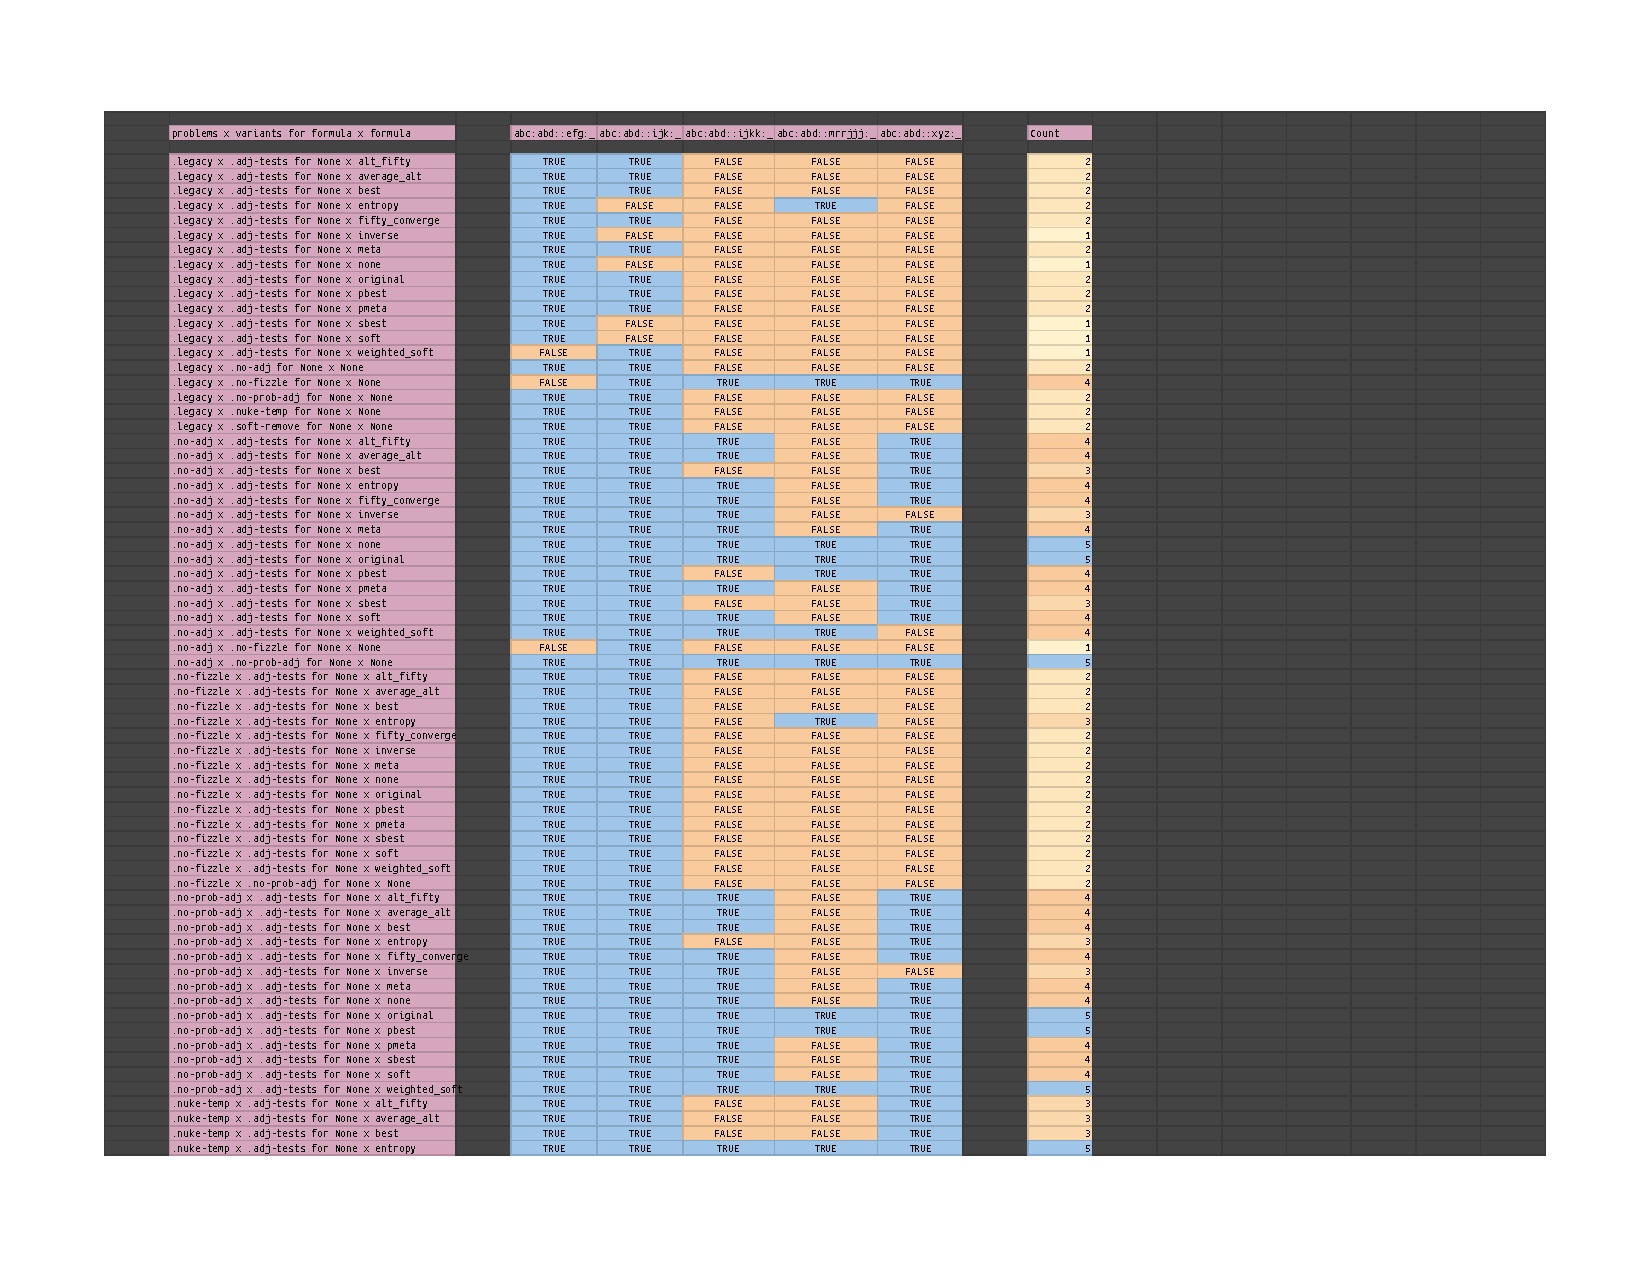
\includepdf[pages={-}]{resources/final.pdf}

\section{Discussion}

    \subsection{Distributed Computation Accuracy}

        [Summary of introduction, elaboration based on results]

    \subsection{Prediction}

        Even though imperative, serial, centralized code is turing complete just like functional, parallel, distributed code, I predict that the most progressive cognitive architectures of the future will be created using functional programming languages that run distributedly and in true parallel. 
        I also predict that, eventually, distributed code will be run on hardware closer to the architecture of a GPU than of a CPU.

\bibliographystyle{alpha}
\bibliography{sample}

\end{document}
